% Copyright 2016 - 2019 Bas van Meerten and Wouter Franssen
%
%This file is part of ssNake.
%
%ssNake is free software: you can redistribute it and/or modify
%it under the terms of the GNU General Public License as published by
%the Free Software Foundation, either version 3 of the License, or
%(at your option) any later version.
%
%ssNake is distributed in the hope that it will be useful,
%but WITHOUT ANY WARRANTY; without even the implied warranty of
%MERCHANTABILITY or FITNESS FOR A PARTICULAR PURPOSE.  See the
%GNU General Public License for more details.
%
%You should have received a copy of the GNU General Public License
%along with ssNake. If not, see <http://www.gnu.org/licenses/>.

\documentclass[11pt,a4paper]{article}
% Copyright 2016 - 2017 Bas van Meerten and Wouter Franssen
%
%This file is part of ssNake.
%
%ssNake is free software: you can redistribute it and/or modify
%it under the terms of the GNU General Public License as published by
%the Free Software Foundation, either version 3 of the License, or
%(at your option) any later version.
%
%ssNake is distributed in the hope that it will be useful,
%but WITHOUT ANY WARRANTY; without even the implied warranty of
%MERCHANTABILITY or FITNESS FOR A PARTICULAR PURPOSE.  See the
%GNU General Public License for more details.
%
%You should have received a copy of the GNU General Public License
%along with ssNake. If not, see <http://www.gnu.org/licenses/>.

\usepackage[british]{babel}
\usepackage{graphicx,booktabs,listings,amsmath,pgfplots,pgfplotstable}
\usepackage[small,bf,nooneline]{caption}
\usepackage{subcaption}
\usepackage[sort&compress,numbers]{natbib}
\usepackage{tikz}
\usepackage{mathtools}
\usepackage[nottoc]{tocbibind}%adds bibliography to table of contents.
\graphicspath{{./images/}}
%\setlength{\textwidth}{453pt} %597 pt is the a4 paperwidth. Minus 2 in margin. 72 pt = 1 in
%\setlength{\hoffset}{-\oddsidemargin}
%\setlength{\voffset}{-30pt} %
%\setlength{\textheight}{651 pt} %a4 height 845 pt minus 2* total headheight. In this case 2*88pt
%% examine margines via the layout package. Use command \layout{} in document to draw a picture.
%\setlength{\parindent}{0.5 cm}
%\setlength{\parskip}{0 cm}
\usepackage[left=82pt,right=82pt,top=95pt,bottom=95pt,footnotesep=0.5cm]{geometry}
%\setlength{\headheight}{14pt}

%define colours--------------------
%dark
\usepackage{xcolor}
\definecolor{MyGrayD}{RGB}{1,1,1}
\definecolor{MyRedD}{RGB}{237,45,46}
\definecolor{MyGreenD}{RGB}{0,140,71}
\definecolor{MyBlueD}{RGB}{24,89,169}
\definecolor{MyOrangeD}{RGB}{243,125,34}
\definecolor{MyPurpleD}{RGB}{102,44,145}
\definecolor{MyBrownD}{RGB}{161,29,32}
\definecolor{MyPinkD}{RGB}{179,56,147}
%normal
\definecolor{MyGray}{RGB}{114,114,114}
\definecolor{MyRed}{RGB}{241,89,95}
\definecolor{MyGreen}{RGB}{121,195,106}
\definecolor{MyBlue}{RGB}{89,154,211}
\definecolor{MyOrange}{RGB}{249,166,90}
\definecolor{MyPurple}{RGB}{158,102,171}
\definecolor{MyBrown}{RGB}{205,112,88}
\definecolor{MyPink}{RGB}{215,127,179}
%light
\definecolor{MyGrayL}{RGB}{204,204,204}
\definecolor{MyRedL}{RGB}{242,174,172}
\definecolor{MyGreenL}{RGB}{216,228,170}
\definecolor{MyBlueL}{RGB}{184,210,235}
\definecolor{MyOrangeL}{RGB}{242,209,176}
\definecolor{MyPurpleL}{RGB}{212,178,211}
\definecolor{MyBrownL}{RGB}{221,184,169}
\definecolor{MyPinkL}{RGB}{235,191,217}
%----------------------------------

%Figure ref with hyperref
\newcommand{\fref}[1]{\hyperref[#1]{Figure \ref*{#1}}}
\newcommand{\sref}[1]{\hyperref[#1]{Section \ref*{#1}}}
\newcommand{\tref}[1]{\hyperref[#1]{Table \ref*{#1}}}

%Makes a new command for figures with input values: filename, width(times linewidth),
% caption and label.
\newcommand{\onefigure}[4]{
\setlength{\captionwidth}{#2\linewidth}
\begin{figure}
\includegraphics[width=#2\linewidth]{#1}
\centering
\parbox{\linewidth}{\caption{#3}
\label{#4}}
\end{figure}
}

%Makes a new command for tikz figures with input values: tikz commands, 
% caption and label.
\newcommand{\onetikz}[3]{
\settowidth{\captionwidth}{#1}
\ifthenelse{\lengthtest{\captionwidth<0.7\linewidth}}{\setlength{\captionwidth}{0.7\linewidth}}{}

\begin{figure}
\centering
#1
\centering
\parbox{\linewidth}{\caption{#2}
\label{#3}}
\end{figure}
}

%Makes a new command for two figures next to each other with input values: filename1, caption1, label1,filename2, caption2 and label2. Figure width is set to 0.47\linewidth and the space between the figures is filled with \hfill so the sides of the figures align with to edge of the line.
\newcommand{\twofigure}[6]{
\setlength{\captionwidth}{\linewidth}
\begin{figure*}[ht!]
\begin{minipage}[t]{0.47\linewidth}
\includegraphics[width=\linewidth]{#1}
\centering
\caption{#2}
\label{#3}
\end{minipage}
\hfill
\begin{minipage}[t]{0.47\linewidth}
\centering
\includegraphics[width= \linewidth]{#4}
\centering
\caption{#5}
\label{#6}
\end{minipage}
\end{figure*}
}


%Makes a new command for a table with caption witdh equal to the total table width. Input: tabular, caption and label. Example:
%\onetable{
%\begin{tabular}{ccc}
%a&b&c\\
%\hline
%1&1&1\\
%1&1&1\\
%1&1&1\\
%\end{tabular}
%{The caption.}
%{tab:table1}
%}
\newcommand{\onetable}[3]{
\settowidth{\captionwidth}{#1}
\ifthenelse{\lengthtest{\captionwidth<0.7\linewidth}}{\setlength{\captionwidth}{0.7\linewidth}}{}
\begin{table}
\caption{#2}
\vspace{-0.24cm} %Puts caption close to toprule
\label{#3}
\centering
#1
\end{table}
}

%Makes a long table with captionwidth equal to tablewidth. It takes the following arguments:
%1: Column specifier (e.g. cccc)
%2: Caption
%3: Label
%4: First head (i.e. first row of regular table)
%5: Head of consecutive pages
%6: Foot of pagebreak
%7: Lastfoot (e.g. \midrule)
%8: Body of table
\newcommand{\onelongtable}[8]{
\begin{center}
\settowidth{\captionwidth}{
\begin{tabular}{#1}
#4
#8
\end{tabular}} % This ends the captionwidth part. Next comes the real table.

\begin{longtable}{#1}
\caption{#2}\\
\vspace{-0.74cm} %Puts caption close to toprule
\label{#3}\\

#4
\endfirsthead

#5
\endhead

#6
\endfoot

#7
\endlastfoot

#8
\end{longtable}
\end{center}}




%1:pgfplots code
%2:width
%3:caption
%4:label
\newcommand{\pgfplotsfigure}[4]{
\pgfplotsset{width=#2\linewidth}
\setlength{\captionwidth}{#2\linewidth}
\begin{figure}[t]
\centering
#1
\centering
\parbox{\linewidth}{\caption{#3}
\label{#4}}
\end{figure}
}


\usepackage[bitstream-charter]{mathdesign}
\usepackage[T1]{fontenc}
\usepackage[protrusion=true,expansion,tracking=true]{microtype}
\pgfplotsset{compat=1.7,/pgf/number format/1000 sep={}, axis lines*=left,axis line style={gray},every outer x axis line/.append style={-stealth'},every outer y axis line/.append style={-stealth'},tick label style={font=\small},label style={font=\small},legend style={font=\footnotesize}}
\usepackage{colortbl}
\usetikzlibrary{calc}

%Set section font
\usepackage{sectsty}
\allsectionsfont{\color{black!70}\fontfamily{SourceSansPro-LF}\selectfont}
%--------------------


%Set toc fonts
\usepackage{tocloft}
%\renewcommand\cftchapfont{\fontfamily{SourceSansPro-LF}\bfseries}
\renewcommand\cfttoctitlefont{\color{black!70}\Huge\fontfamily{SourceSansPro-LF}\bfseries}
\renewcommand\cftsecfont{\fontfamily{SourceSansPro-LF}\selectfont}
%\renewcommand\cftchappagefont{\fontfamily{SourceSansPro-LF}\bfseries}
\renewcommand\cftsecpagefont{\fontfamily{SourceSansPro-LF}\selectfont}
\renewcommand\cftsubsecfont{\fontfamily{SourceSansPro-LF}\selectfont}
\renewcommand\cftsubsecpagefont{\fontfamily{SourceSansPro-LF}\selectfont}
%--------------------


\usepackage[hidelinks,colorlinks,allcolors=black, pdftitle={Multiple quadrupolar pattern fitting in ssNake},pdfauthor={Wouter M.J.\ Franssen}]{hyperref}

\interfootnotelinepenalty=10000 %prevents splitting of footnote over multiple pages
\linespread{1.2}

\title{\color{black}\fontfamily{SourceSansPro-LF}\bfseries Multiple quadrupolar pattern fitting in ssNake}
\author{}
\date{\color{black}\fontfamily{SourceSansPro-LF}\bfseries \today}


\begin{document}
%\newgeometry{left=72pt,right=72pt,top=95pt,bottom=95pt,footnotesep=0.5cm}
\microtypesetup{protrusion=true} % enables protrusion

\maketitle

\section{Introduction}
Is this tutorial, I will demonstrate how to fit multiple spectra at the same time with linked
parameters. The example that we will treated here is for second order quadrupolar patterns. These
patterns scale in width as a function of the magnetic field. In some cases, the occurrence of
multiple atomic sites complicates a correct fitting of these line shapes. The aid with the fitting
of these spectra, additional data is often recorded at different magnetic fields. Fitting these
spectra simultaneously, linking there quadrupolar parameters, will then lead to a more accurate
fit result.

Before continuing with this tutorial, it might be wise to check out our other tutorial about CSA
fitting, to get acquainted with the fitting procedure in ssNake.

\section{Data}
The data used in this tutorial are $^{87}$Rb spectra of rubidium nitrate (RbNO$_3$) powder which was recorded on a
Varian 300 MHz and 850 MHz spectrometer. 25 kHz MAS was used for both spectra.

\section{Fitting a single quadrupole spectrum}
As a start, we will load one of the spectra, and fit that one on its own.

\begin{itemize}
  \item Load the `850MHz.mat' file that was delivered with this tutorial
  \item Put the x-axis on `ppm' (via the `Axis' dropdown in the bottomframe)
\end{itemize}
This should show:
\begin{center}
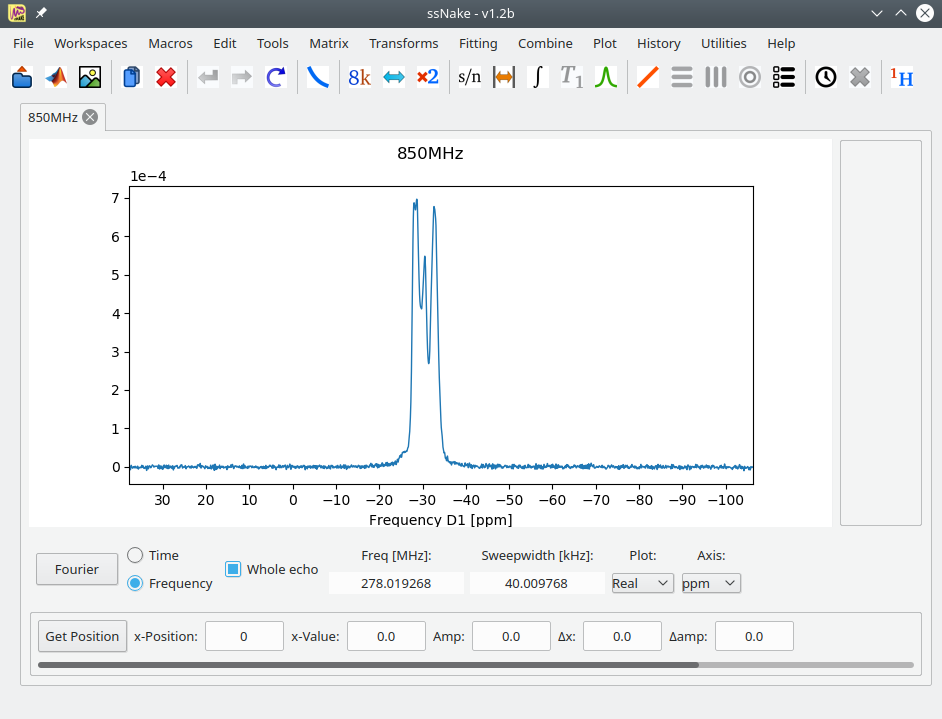
\includegraphics[width=0.8\linewidth]{Figs/Fig1.png}
\end{center}

Now we go to the fitting:

\begin{itemize}
  \item Fitting $\longrightarrow$ Quadrupole
\end{itemize}
This shows the fitting window (I zoomed the x-axis for this Figure):

\begin{center}
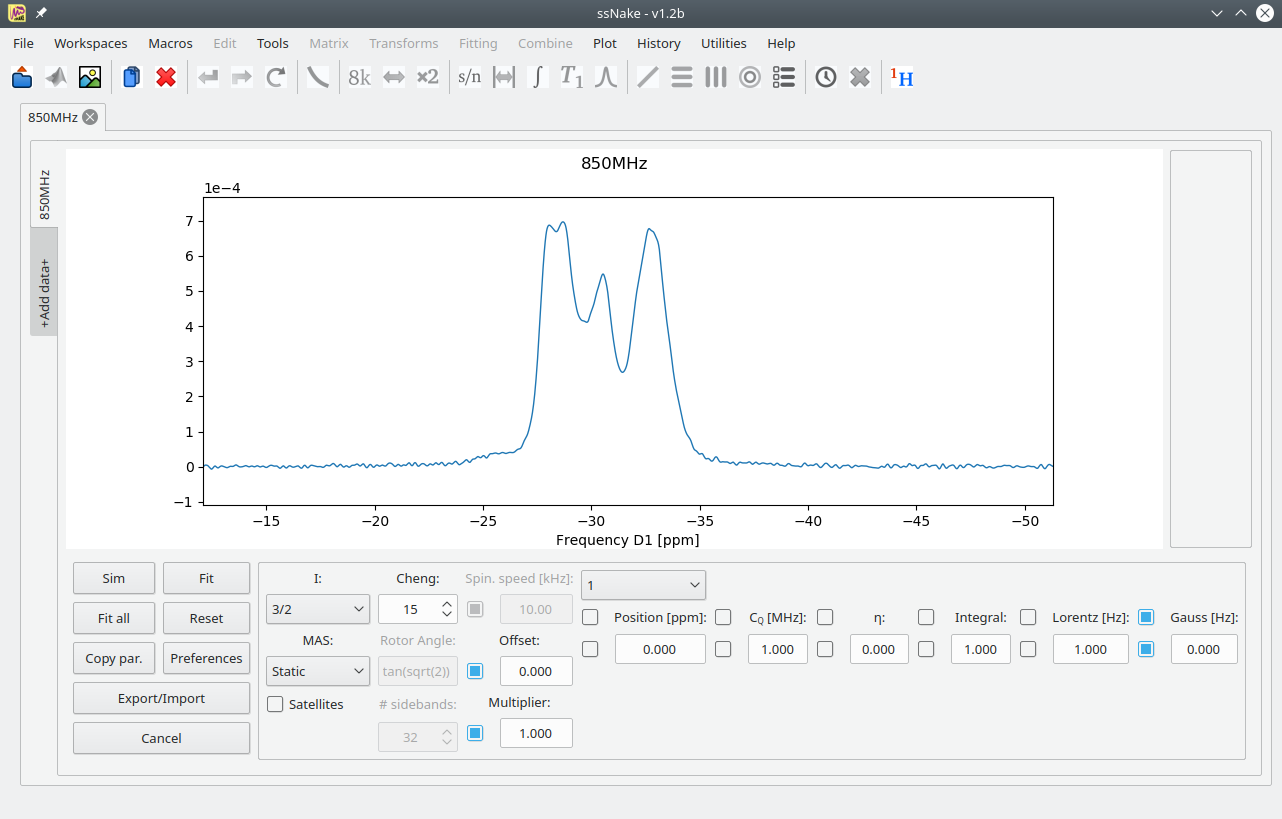
\includegraphics[width=1.0\linewidth]{Figs/Fig2.png}
\end{center}

Firstly, we must make sure that some general settings are correct. $^{87}$Rb is a spin 3/2 nucleus, so
$I$ should be 3/2 (this is the default value). The MAS settings should be at 'Infinite MAS', and the
satellites should be turned off\footnote{The 25 kHz MAS that was used in the experiment is fast enough
for the central transition to be considered infinite. The satellite transition are ignored, as they
are not properly excited in this experiment anyhow.}.

This gives:
\begin{center}
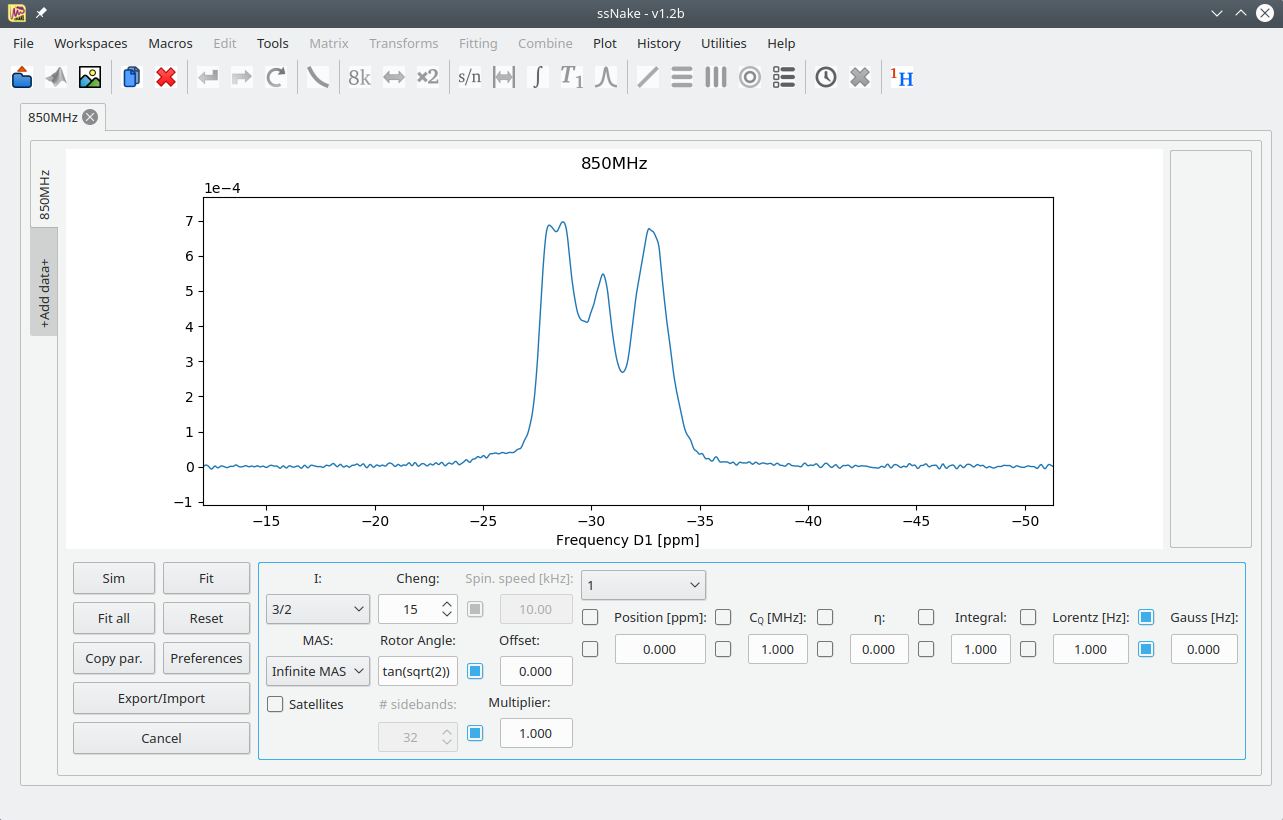
\includegraphics[width=1.0\linewidth]{Figs/Fig3.png}
\end{center}

Now, we can start by filling in some starting values for the fit. These can be tricky to establish, so we
will just use the literature values in this case (i.e. from the ssNake paper).

\begin{center}
  \begin{tabular}{cccc}
	 \toprule
	 Site & Position [ppm] & $C_\text{Q}$ [MHz] & $\eta$\\
	 \midrule
	 1 & $-27.41$ & 1.687 & 0.17\\
	 2 & $-28.71$ & 1.984 & 1.0\\
	 3 & $-31.82$ & 1.711 & 0.58\\
	 \bottomrule
  \end{tabular}
\end{center}
Filling this in leads to:
\begin{center}
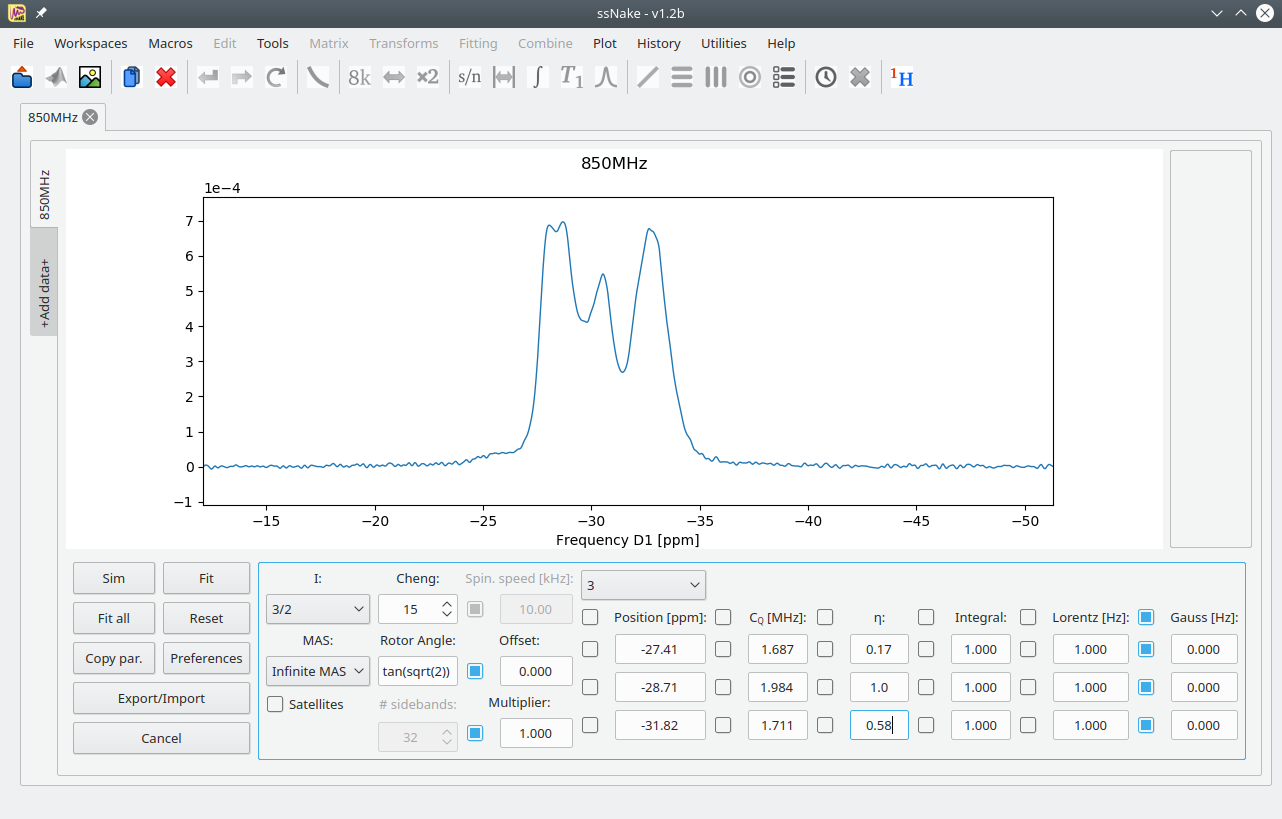
\includegraphics[width=1.0\linewidth]{Figs/Fig4.png}
\end{center}

One thing we have to deicide now, is how we are going to consider the three different sites in
RbNO$_3$. In principle, these should have the same integral. In this case, we will force this
equality in our fit. We do this by fixing all of their integrals at 1. We then use the `Multiplier'
parameter to do the scaling to get the intensities of our simulation equal to the experiment.

Now we can do an initial simulation, to so how that goes. Pushing `Sim' gives:
\begin{center}
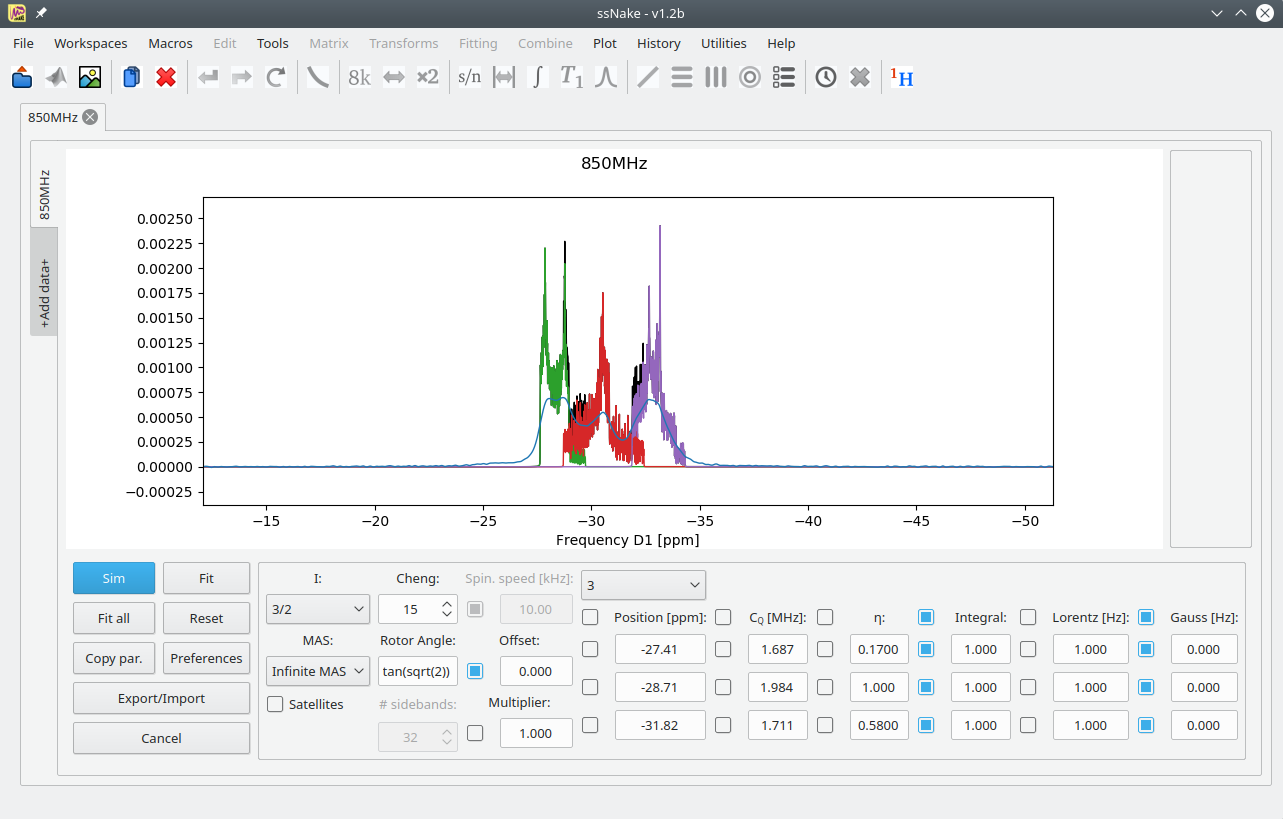
\includegraphics[width=1.0\linewidth]{Figs/Fig5.png}
\end{center}
We notice multiple thing: the simulation looks very sharp, so we need some line broadening, and the
intensities are a bit high.
\begin{itemize}
  \item Put all `Lorentz' values at 100 Hz
  \item Put the `Multiplier' at 0.8
\end{itemize}
This looks much better:
\begin{center}
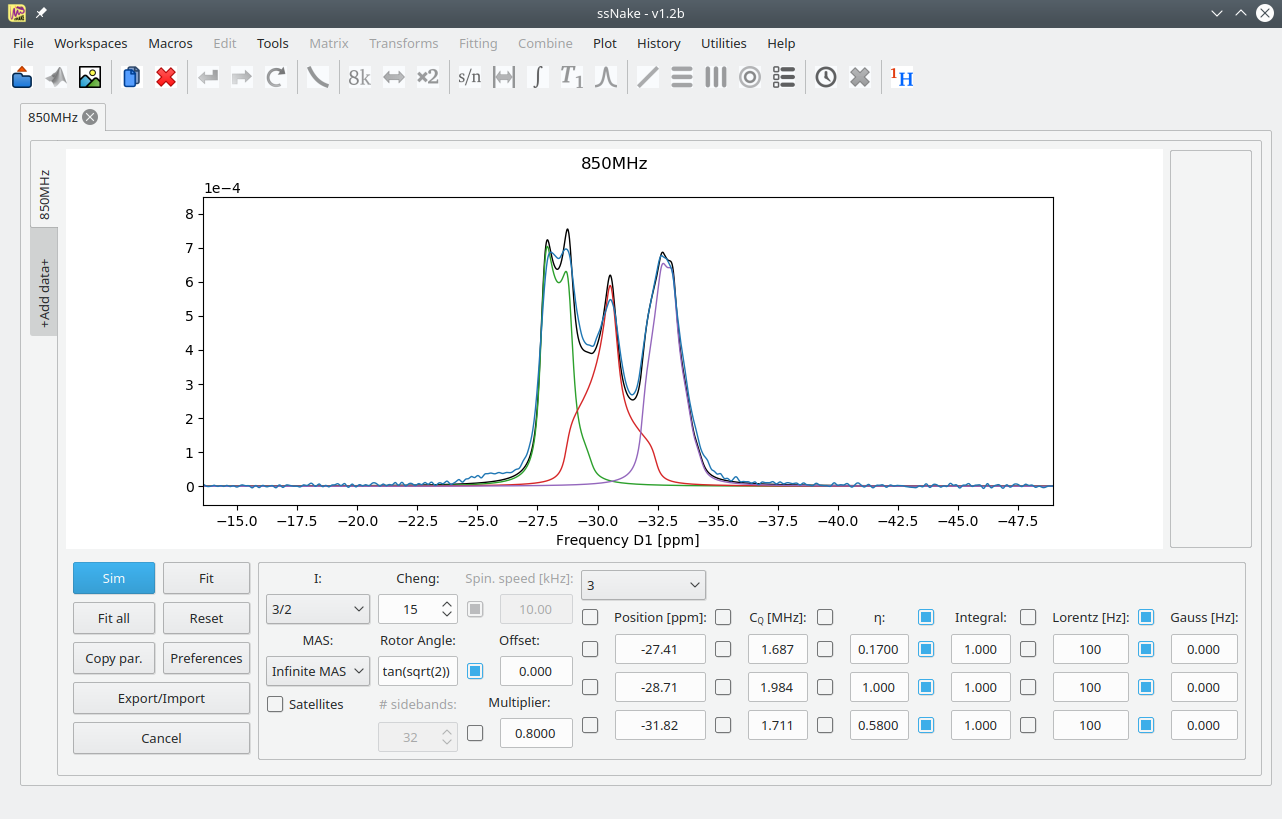
\includegraphics[width=1.0\linewidth]{Figs/Fig6.png}
\end{center}
Now we can fit and see where this goes. Push `Fit' and observe (after some seconds):
\begin{center}
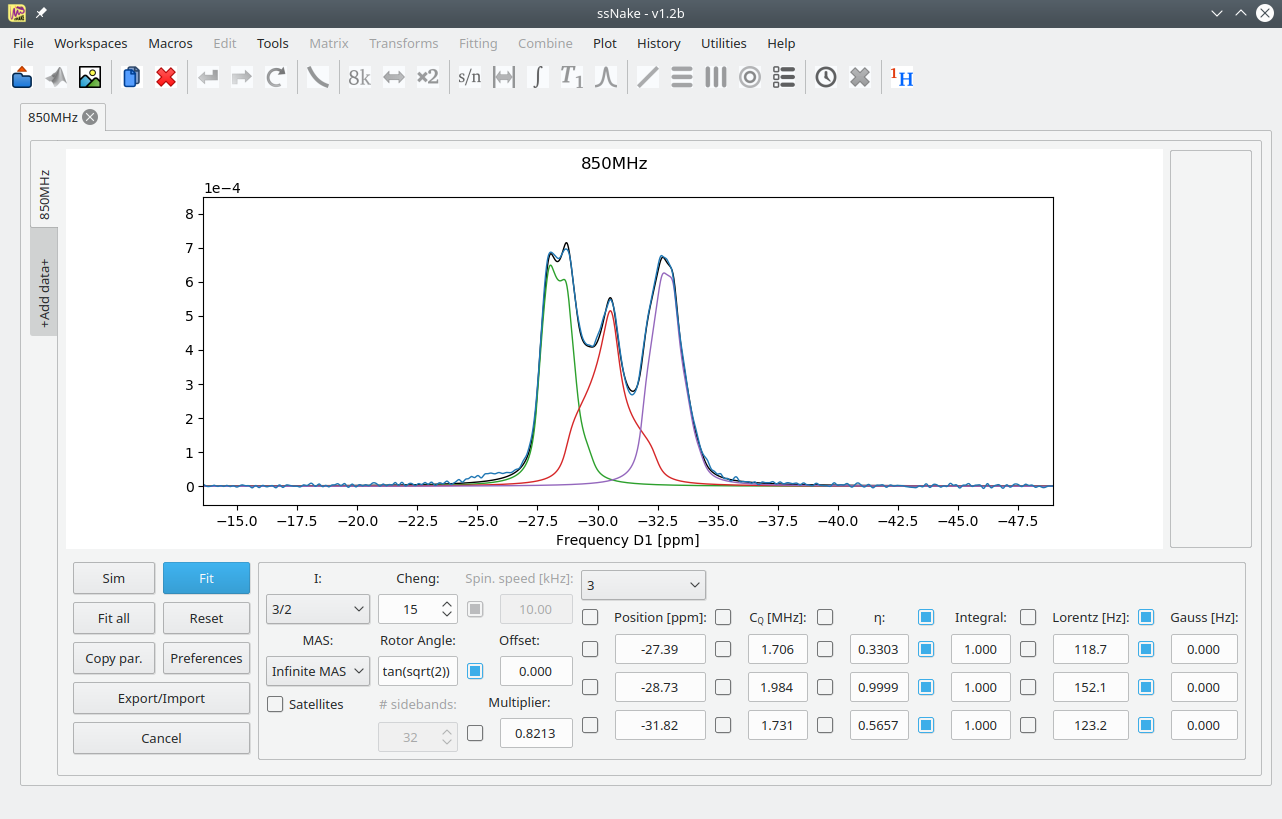
\includegraphics[width=1.0\linewidth]{Figs/Fig7.png}
\end{center}
This looks like a nice fit! The parameters only changed slightly, as we cheated by putting in the
right values at the start. Observe that we do not describe the intensity around $-25$ ppm: this is
the centre band of the satellites, which we do not include in the simulation (see the ssNake paper
for a solution on how to include these).

Now we continue by adding extra data, to fit simultaneously.

\section{Fitting multiple spectra simultaneously}
\begin{itemize}
  \item Load the `300.mat' file that was delivered with this tutorial
  \item Put the x-axis on `ppm' (via the `Axis' dropdown in the bottomframe)
\end{itemize}

Now, we are going to add this data to the fit:
\begin{itemize}
  \item Go to the 850MHz workspace
  \item Click `+Add data+' in the vertical tabbar
  \item Select the 300MHz workspace and push `OK'
\end{itemize}
This gives us the extra data in a new fitting tab. Note that we do not have all the options present
in the left hand side of the parameters. These are only available in the master fit tab (i.e. the
850MHz tab). 

We start by setting some parameters right:
\begin{itemize}
  \item Set MAS to `Infinite MAS'
  \item Set the number of sites to 3 (via the dropdown menu)
  \item Set all Lorentz values at 100 Hz
  \item Fix the integrals at 1
  \item Unfix the `Multiplier'
\end{itemize}
This gives:
\begin{center}
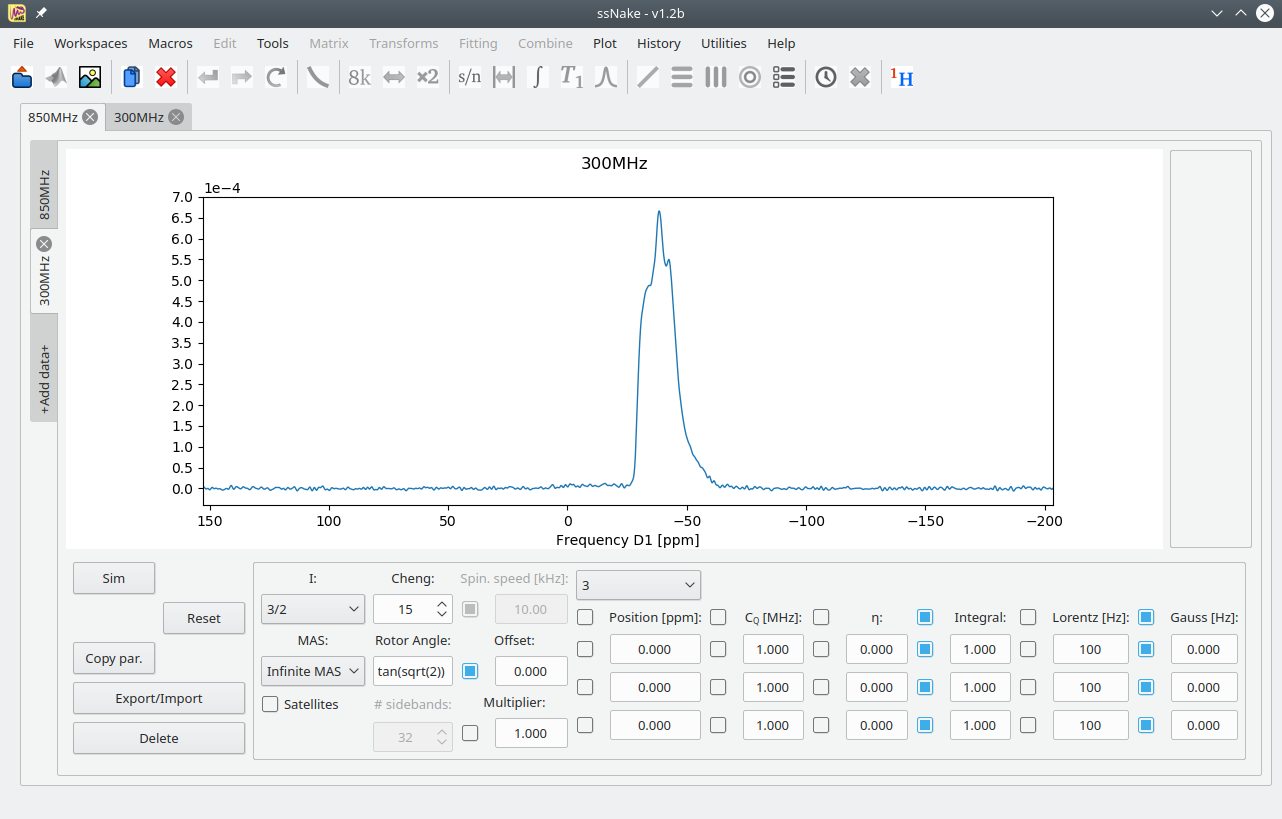
\includegraphics[width=1.0\linewidth]{Figs/Fig8.png}
\end{center}

Now for the important part: linking parameters. As we are observing the same sample in both data sets,
the position, $C_\text{Q}$ and $\eta$ are identical in both spectra. We can do this by right
clicking on a parameter input box, and use `Connect parameter'. Do this for the first `Position'
entry. This gives the following input
window:
\begin{center}
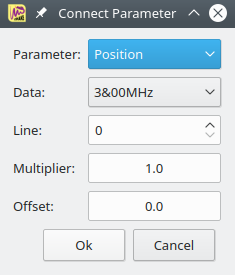
\includegraphics[width=0.3\linewidth]{Figs/Fig9.png}
\end{center}
This has the following parameters:
\begin{itemize}
  \item Parameter: The name of the parameter that we want to link to
  \item Data: the name of the data tab that we want to link to
  \item Line: the line (i.e. sites) the we want to link to (`0' is the first, as everywhere in
	 ssNake)
  \item Multiplier: multiplier the linked value by this value
  \item Offset: offset the linked value with this amount
\end{itemize}
 In our case, we want our parameter (the first `Position' of the 300MHz data) to be linked to the
 first `Position' of the 850 MHz data. We do not need a scaling ($\text{Mutiplier}=1.0$) or offset.

 Set properly, this gives\footnote{Ignore the \& signs in the `Data' names. This is a bug at the
 moment\ldots}:
\begin{center}
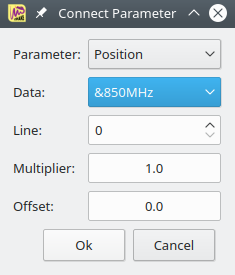
\includegraphics[width=0.3\linewidth]{Figs/Fig10.png}
\end{center}
Pushing `Ok' prints `('Position', 0, 1.0, 0.0, 0)' in the box we selected with our right mouse button
before. The input represents: ('Par name', Line, Multiplier, Offset, Data index). The pop-up menu we
used is essentially an easy tool to create this input. Now, this value is linked, to be identical to
the first Position value of the 850MHz data.

We can now do the same for the other `Position' values, linking the to Lines 1 and 2 of the 850MHz
data:
\begin{itemize}
  \item Set the second position value to: ('Position', 1, 1.0, 0.0, 0)
  \item Set the third position value to: ('Position', 2, 1.0, 0.0, 0)
\end{itemize}

We can now do the same for the $C_\text{Q}$ and $\eta$ values, linking them to the 805MHz
parameters. Note that the names of the parameters are not always equal to those labeled above the
input boxes. $\eta$ is named `eta' for example. After linking all paramters, we should have the
following:
\begin{center}
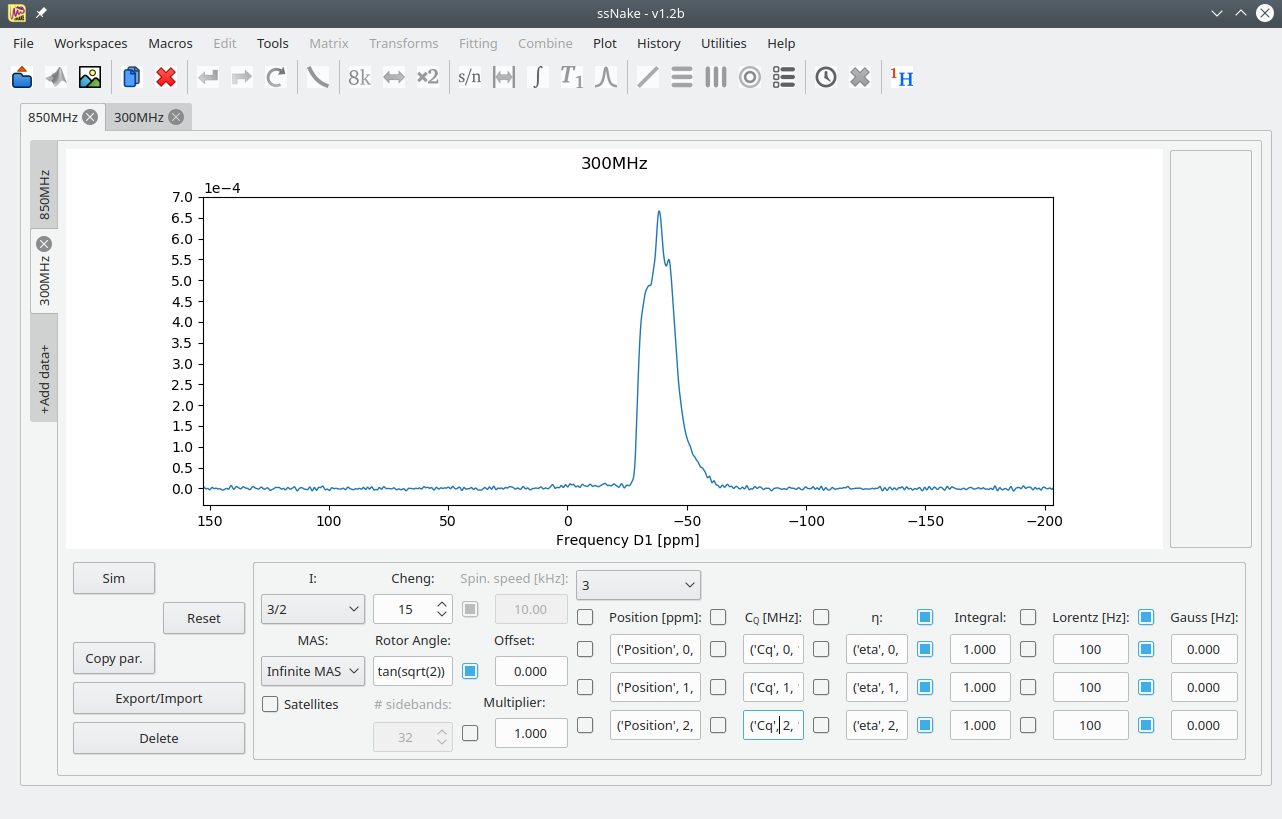
\includegraphics[width=1.0\linewidth]{Figs/Fig11.png}
\end{center}
Now, we can push `Sim' to do a simulation:
\begin{center}
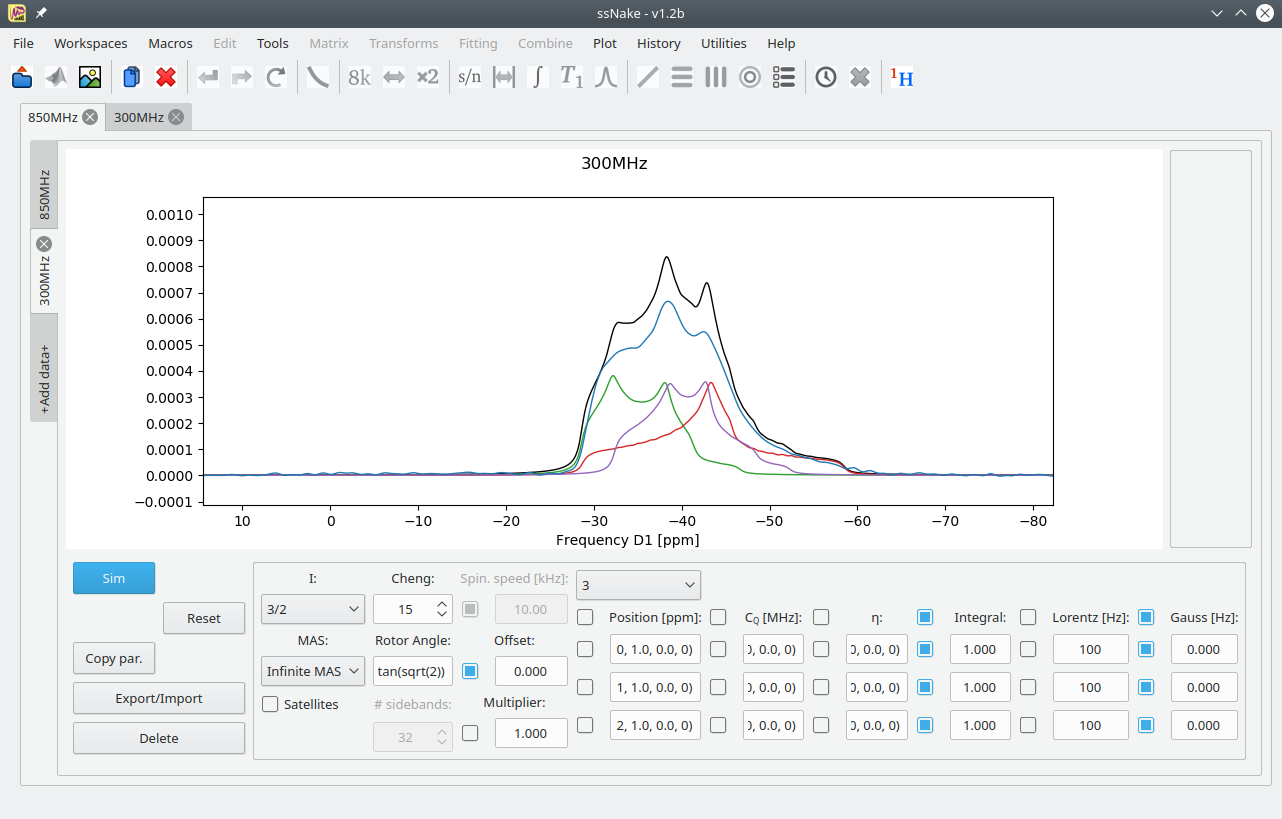
\includegraphics[width=1.0\linewidth]{Figs/Fig12.png}
\end{center}
This gives a nice spectrum. Clearly the linking succeeded, otherwise we would not be able to simulate
a spectrum without having any $C_\text{Q}$ and eta values.

Now, we should be ready for a fit! Go back to the `850MHz' fitting tab, and push `Fit'. This will
take some time, as we now have to calculate six powder patterns per iteration.

The 300MHz data for me now shows:
\begin{center}
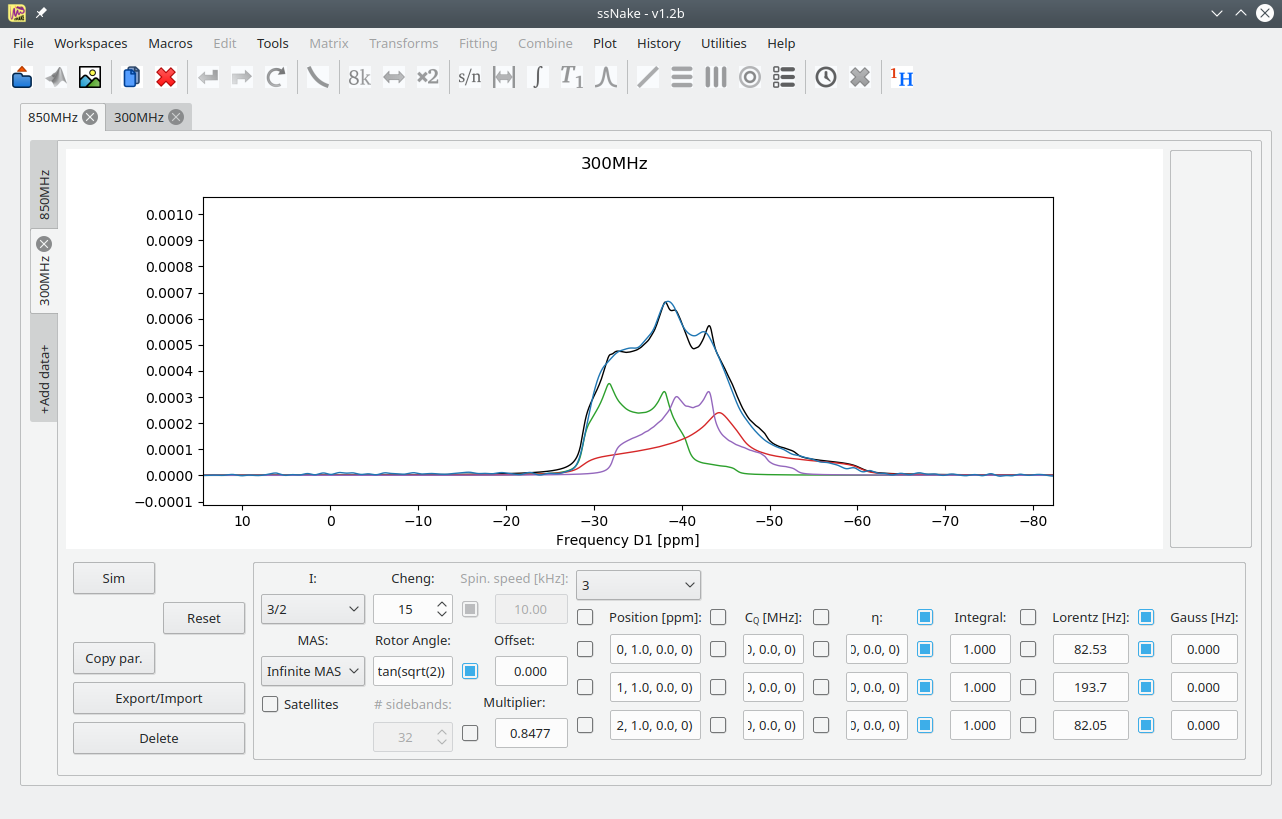
\includegraphics[width=1.0\linewidth]{Figs/Fig13.png}
\end{center}
This is ok, but not great. Probably we need some Gaussian broadening for this line:
\begin{itemize}
  \item Untick the Gaussian boxes and set them to 50 Hz
  \item Fit again
\end{itemize}
Which leads to:
\begin{center}
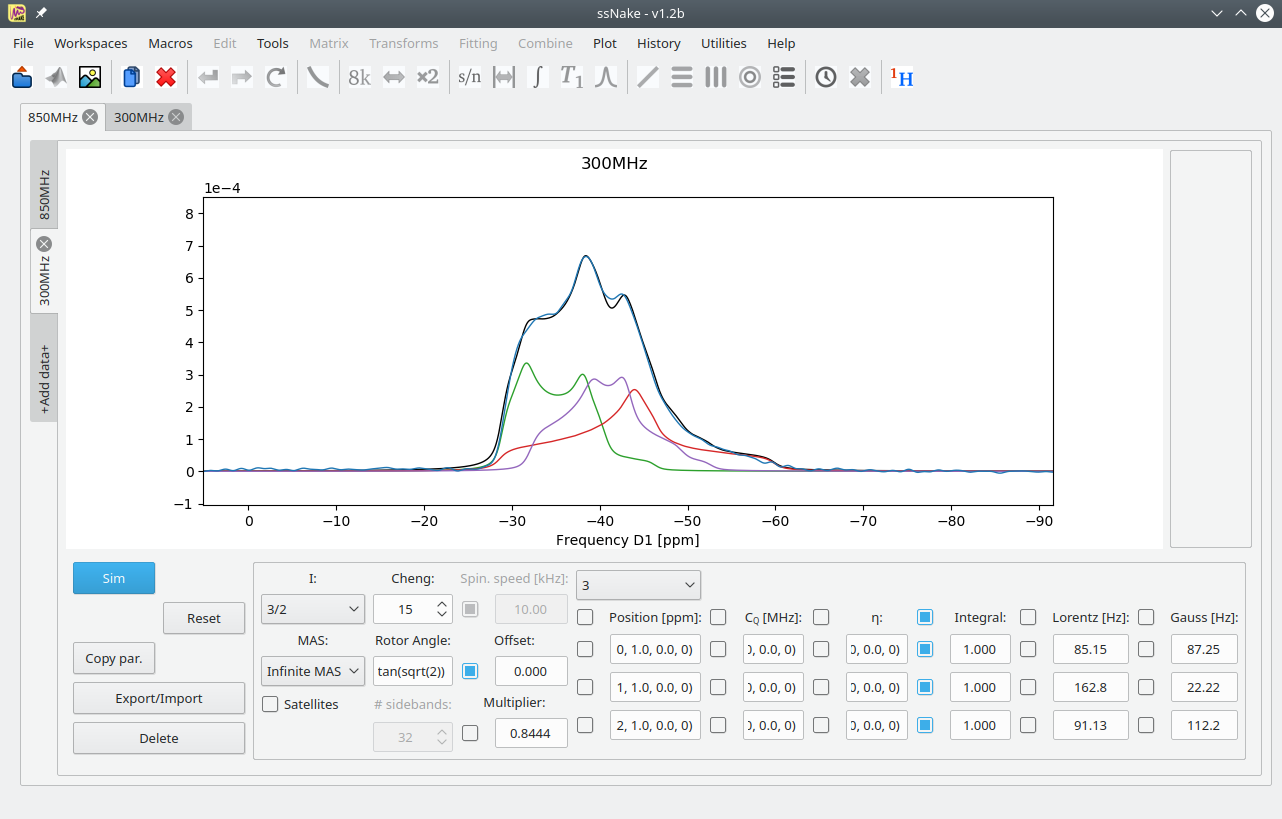
\includegraphics[width=1.0\linewidth]{Figs/Fig14.png}
\end{center}
which looks much better. We have therefore succeeded in doing a simultaneous fit! Fitting the data
with or without the extra 300MHz data will lead to different results (you can check this yourself).
Hopefully, the fit with the extra data is more accurate\ldots Supplied with this tutorial are
additional spectra recorded at 400 and 600 MHz. If you like you can replicate the 4 spectra fit that
was demonstrated in the ssNake paper.

\section{Do's and don'ts}
When fitting multiple spectra simultaneously, we must make sure that the parameters like the
quadrupolar parameters \textit{are} indeed identical in all spectra. Be careful with temperature
changes (MAS induced heating!), sample degradations, and carefully reference your ppm axis. Changes
like this can actually reduce the overall quality of the fit, when including more data. Especially
when fitting spectra with narrow lines, changes of 0.1 Hz in position can be of considerable
influence. In some cases, we can of course chose not to link some parameters which we know to be
very sensitive to temperature effects. The data in this tutorial was recorded using the same probe (a
850 MHz probe) at four different fields, using the same gas flows and the same reference compound. I
might have overdone it in terms of safety, but then RbNO$_3$ is quite sensitive to temperature changes.

Do not chain-link parameters. This does not work. That is, do not link par2 to par1, and par3 to
par2. Always refer to the original parameter (link par 2 to par1, and par3 to par1). In the future,
this should hopefully give an error message\ldots

Be very careful with the vertical scaling of the spectra. If spectrum1 has 10000x more intensity
than spectrum2, spectrum2 will be almost ignored during the fit. I always scale the spectra to have
the same integral, as was also done for the data in this tutorial. This is often a safe option
(scaling can be done via Matrix $\longrightarrow$ Normalize). However, if one of these spectra has a
lot more noise than the others, you might want to consider lowering its intensity, as to be less
important during the fit. One way to do this is to scale the data to make sure the intensities of
the noise band are equal. Tread carefully\ldots

\end{document}
